\documentclass[12pt]{article}
\usepackage[top= 3cm, bottom=2cm, left=2cm, right=2cm]{geometry}
\usepackage[utf8]{inputenc}
\usepackage{url}
\usepackage{hyperref}
\hypersetup{
    colorlinks=true,
    urlcolor=blue,
    linkcolor=blue,
    citecolor=blue
    }
\usepackage{graphicx}
\usepackage[sorting=none]{biblatex} %Imports biblatex package
\addbibresource{biblio.bib} %Import the bibliography file

\usepackage[breakable]{tcolorbox}
\usepackage{enumerate}
\usepackage[spanish]{babel}
\usepackage{csquotes}
\usepackage{todonotes}

%SIMBOLOS
\usepackage{amsfonts} 
\usepackage{amsmath}
\usepackage{MnSymbol}
\usepackage{wasysym}
\usepackage{marvosym}

\usepackage{amsthm}
\setlength {\marginparwidth }{2cm}

%LISTINGS%%%%%%%%%%%%%%%%%%%%%%%%%%%%%%%%%%
\usepackage{multirow}
\usepackage{xcolor}
\usepackage{listings}
\usepackage{listingsutf8}
\lstset{
  inputencoding=utf8/latin1, % Configura la codificación UTF-8
  extendedchars=true,        % Permite caracteres extendidos
  literate={á}{{\'a}}1 {é}{{\'e}}1 {í}{{\'i}}1 {ó}{{\'o}}1 {ú}{{\'u}}1
}
\usepackage{comment}
\usepackage{courier}
%%%%%%%%%%%%%%%%%% LISTING JAVA %%%%%%%%%%%%%%%%%%%%%%%%%%
% Definición de colores
\definecolor{dkgreen}{rgb}{0,0.6,0}
\definecolor{gray}{rgb}{0.5,0.5,0.5}
\definecolor{mauve}{rgb}{0.58,0,0.82}
\definecolor{gray97}{gray}{.97}

% Estilo para el lenguaje Java
\lstdefinestyle{java}{
  frame=Ltb,
  language=Java,
  framerule=0pt,
  rulesep=.4pt,
  backgroundcolor=\color{gray97},
  rulesepcolor=\color{black},
  aboveskip=3mm,
  belowskip=3mm,
  showstringspaces=false,
  columns=flexible,
  basicstyle=\small\ttfamily,
  numbers=left,
  numberstyle=\tiny\color{gray},
  keywordstyle=\color{blue},
  commentstyle=\color{dkgreen},
  stringstyle=\ttfamily\color{mauve},
  breaklines=true,
  breakatwhitespace=true,
  tabsize=3,
  morekeywords={String, ArrayList, MyClass, Exception, IOException} % Agrega aquí los tipos de datos y excepciones adicionales
}

% Configuración adicional para resaltar palabras clave
\lstset{
  emph={numero, identificador, not, true, false, +, -, *, div, or, and, program, var, procedure, function, integer, boolean, begin, end, :=, if, then, else, while, do, =, <, >, \geq, \leq, ;},
  emphstyle=\textbf,
  mathescape=true,
  basicstyle=\ttfamily,
  keywordstyle=\bfseries,
  breaklines=true,
  breakatwhitespace=true
}
%%%%%%%%%%%% FIN CONFIG JAVA LST %%%%%%%%%%%%%%%%%%%%%%%


%%%%%%%%%%%%%%CONFIG SPARQL LST%%%%%%%
\lstdefinelanguage{SPARQL}{
  basicstyle=\small\ttfamily,
  backgroundcolor=\color{white},
  columns=fullflexible,
  breaklines=false,
  sensitive=true,
  % --------------------------
  frame=bt,
  aboveskip=1em,
  belowskip=1em,
  xleftmargin=.5em,
  xrightmargin=.5em,
  framexleftmargin=.5em,
  framextopmargin=.5em,
  framexbottommargin=.5em,
  framexrightmargin=.5em,
  % --------------------------
  tabsize = 2,
  showstringspaces=false,
  morecomment=[l][\color{brown}]{\#},       % comments
  morecomment=[n][\color{teal}]{<http}{>}, % uris
  morestring=[b][\color{magenta}]{"},  % strings
  % -------------------------- variables
  keywordsprefix=?,
  classoffset=0,
  keywordstyle=\color{blue},
  morekeywords={},
  % -------------------------- prefixes
  %todo Aca se configuran las palabras que se quieren poner naranja
  classoffset=1,
  keywordstyle=\color{orange},
  morekeywords={rdf,rdfs,owl,xsd,purl, foaf, wd, wdt,ex, dbpediaOnt,schema, dbpediaPage, dbpediaRes},
  % -------------------------- keywords
  classoffset=2,
  keywordstyle=\color{purple},
  morekeywords={
    SELECT,CONSTRUCT,DESCRIBE,ASK,WHERE,FROM,NAMED,PREFIX,BASE,OPTIONAL,
    FILTER,GRAPH,LIMIT,OFFSET,SERVICE,UNION,EXISTS,NOT,BINDINGS,MINUS,a, @prefix
  }
}
%%%%%%%%%%%FIN CONFIG SPARQL LST %%%%%%%%%%%%%%%%%%%%%%%
\usepackage{caption}
\DeclareCaptionFormat{listing}{\rule{\dimexpr\textwidth+0pt\relax}{0.4pt}\par\vskip1pt#3}
\captionsetup[lstlisting]{format=listing,singlelinecheck=false, margin=0pt, font={sf},labelsep=space,labelfont=bf}

\renewcommand\lstlistingname{Código}

\DeclareMathVersion{sans}
\SetSymbolFont{operators}{sans}{OT1}{cmbr}{m}{n}
\SetSymbolFont{letters}  {sans}{OML}{cmbrm}{m}{it}
\SetSymbolFont{symbols}  {sans}{OMS}{cmbrs}{m}{n}

\lstnewenvironment{sflisting}[1][]
  {\lstset{\#1}\mathversion{sans}}{}
%%%%%%%%%%%%%%%%%%%%%%%%%%%%%%%%%%%%%%%%%%%%
\usepackage{fancyhdr}
\pagestyle{fancy}

%%%COMPLETAR%%% 
\fancyhead[L]{NOMBRE TP}
\fancyhead[R]{NOMBRE MATERIA}


\begin{document}
\begin{titlepage}
  \title{\textbf{NOMBRE MATERIA}\\
  %\vspace{2mm}
  \large{\textbf{TITULO PRACTICO}}
  %\vspace{3mm}
  \author{
  Manuel Latorre FAI-1931\\ manuel.latorre@est.fi.uncoma.edu.ar\vspace{3mm}\\
  }}
  \date{Segundo cuatrimestre 2023}

  \pagenumbering{gobble}
  \maketitle
  \vspace{25mm}
  \vfill
  \hspace*{-0.1in}{
  
\includegraphics[width=7cm, scale=0.5]{Images/Unco/faiLogo.png}
  \hspace*{1.5in}
  
\includegraphics[width=5cm, scale=0.5]{Images/Unco/Unco logo.png}
  }
\end{titlepage}

\titlepage

\newpage

\pagebreak

%INDICE Y FIGURAS
\newpage
\tableofcontents %%Indice
\listoffigures
\clearpage\pagenumbering{arabic}
\newpage

%INPUTS
\section{Definicion de IA}

\begin{figure}
  \centering
  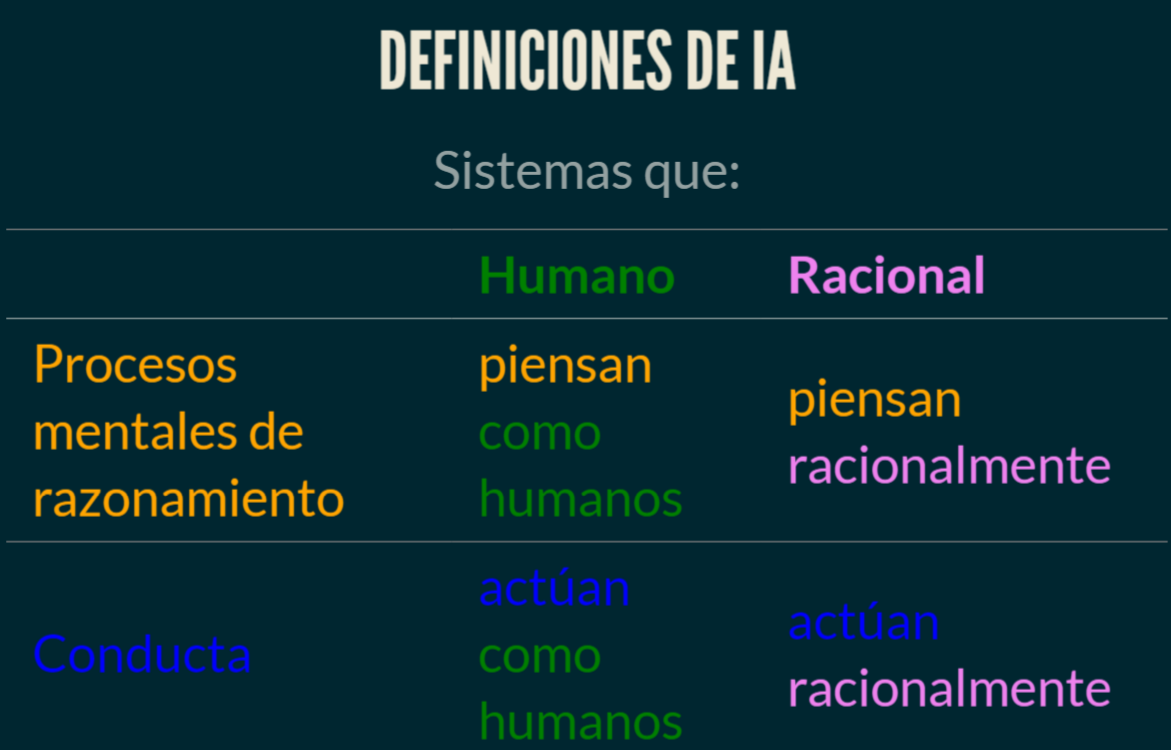
\includegraphics[width=16cm, scale=1]{Images/Imagenes/cuadro1.png}
  \caption{Definiciones de IA}
  \label{fig:marcado}
\end{figure}

\begin{itemize}
  \item \textbf{Piensan como humanos:} Requiere de teorías científicas de las actividades internas del cerebro. Para lograrlo hay que determinar como es que piensan los humanos.
  \item \textbf{Piensan racionalmente:} ir al cap 1 de \cite{sabharwal2011s}
  \item \textbf{Actúan como humanos: }El modelo es el hombre; el objetivo es construir un sistema que se haga pasar por un humano.
  
  Turing propone un Test operacional para el funcionamiento inteligente, las capacidades necesarias son:
  \begin{itemize}
    \item Procesamiento de lenguaje natural
    \item Representación del conocimiento
    \item Razonamiento
    \item Aprendizaje
  \end{itemize}
  El Test consiste en un juez realizando preguntas a dos participantes (X e Y) que no puede ver: un hombre y una mujer. El juez debe averiguar, por medio de preguntas quien es el hombre y quien la mujer. Los participantes pueden mentir o tratar de engañar al juez
  \item \textbf{Actúan racionalmente (este es el que nos interesa):} El comportamiento racional hace referencia a realizar la acción correcta. Es decir, aquello que se espera maximice la meta a alcanzar, dada la información disponible
\end{itemize}

\textbf{Agente: }Un agente es una entidad que percibe y actúa. Abstractamente, un agente es una función desde historias de percepciones a acciones:

\begin{equation}
  f: P* \rightarrow A 
\end{equation}

Para toda clase de ambientes y tareas, buscamos el agente con la mejor perfomance

\textbf{IA fuerte vs Debil }
\begin{itemize}
  \item \textbf{IA fuerte: }Una maquina que piense debera tener conciencia y mente real
  \item \textbf{IA débil: }Las maquinas podrían actuar como si ellas fueran inteligentes
\end{itemize}

\textbf{Inteligencia artificial vs sintética}
\begin{itemize}
  \item \textbf{Artificial: }Hecho por el hombre. Sugiere que es algo de calidad diferente a lo natural. Por ejemplo, lago artificial, brazo artificial.
  \item \textbf{Sintético: }Producto obtenido por procedimientos mecánicos, electrónicos o industriales y que imita otro producto natural. Por ejemplo césped sintético  
\end{itemize}

\subsection{Agentes}
\todo[inline]{Esta seccion hay que sabersela de memoria, se arrastra hasta el final de la carrera}
Un agente racional es aquel que hace las acciones correctas. Una accion correcta, es aquella que causa que el agente sea mas exitoso.
\begin{itemize}
  \item Una \textbf{secuencia de acciones} afectan al ambiente que pasa por una secuencia de estados. Por ejemplo cuando moves una pieza jugando al ludo, el ambiente es el tablero y tu acción de mover una pieza modifico la configuración de este
  \item \textbf{Medida de performance} criterio objetivo que establece cuan exitoso es el comportamiento del agente. Evalúa cuan deseable es la secuencia de estados del ambiente generados por la secuencia de acciones del agente
\end{itemize}

Las medidas de performance se diseñan de acuerdo a loq ue uno realmente \textbf{quiere en el ambiente} en vez de considerar la forma en que uno piensa que el agente se debería comportar

\textbf{Racionalidad en un agente racional: }en un momento dado depende de:
\begin{itemize}
  \item La medida de performance que define un criterio de éxito
  \item El conocimiento a priori del ambiente
  \item Las acciones que el agente puede ejecutar
  \item La secuencia de percepciones del agente hasta el momento
  \item Para cada posible secuencia de percepciones, un agente racional elige la acción que maximiza el valor esperado de la medida de performance (osea la acción que lo hace mas exitoso) esto lo averigua basándose en la evidencia provista por la secuencia de percepciones y el conocimiento predefinido que el agente tiene
\end{itemize}

\textbf{Agente omnisciente: }es aquel que conoce el resultado real de sus acciones y puede actuar de a cuerdo a ello. Esta es imposible en la realidad ya que $Racionalidad \neq Clarividencia$. El agente racional no requiere omnisciencia porque la elección racional depende de la secuencia de percepciones

\textbf{Como trabaja el agente racional:}
\begin{itemize}
  \item Explora: reúne información antes de elegir la acción adecuada. Ejemplo: Si tenes un robot que tiene que cruzar la calle, tiene que mirar a los dos lados para saber cuando cruzar y que no se la den
  \item Autonomía: Toma decisiones en forma \textbf{independiente}. Sus decisiones y sus acciones están bajo su propio control. Tiene sus propias creencias, deseos e intenciones, es decir, no es sirviente de otros (hace la que le pinta en función a lo que sabe). Si un agente confía en el conocimiento a priori de su diseñador en vez de en sus percepciones entonces se dice que le falta autonomía 
\end{itemize}

\subsection*{Tipos de agentes}
\subsubsection*{Agente reactivo o reflexo simple}
\begin{itemize}
  \item Agentes que simplemente reaccionan por un estimulo del ambiente. Por ejemplo una alarma de seguridad
  \item Selecciona una acción en base a la percepción actual, ignorando el resto de la historia de percepciones (el pasado)
  \item No mantienen ninguna representación explicita interna del ambiente
  \item Las decisiones son implementadas en alguna forma de mapeo directo entre situación-acción o condición-acción
\end{itemize}

Tiene un comportamiento dirigido por el principio de estimulo-respuesta característico de los reflejos de humanos, animales y plantas

\textbf{Ventajas: }
\begin{itemize}
  \item Simplicidad
  \item Tratabilidad computacional
\end{itemize}

\textbf{Limitaciones: }
\begin{itemize}
  \item Solo trabajan bien si la acción correcta puede determinarse en base a la percepción actual (El ambiente tiene que ser totalmente observable)
  \item Posibilidad de loops infinitos bajo ambientes parcialmente observables
  \item Incapacidad de analizar la consecuencia futura de las acciones
  \item Difíciles de escalar
\end{itemize}

\begin{figure}
  \centering
  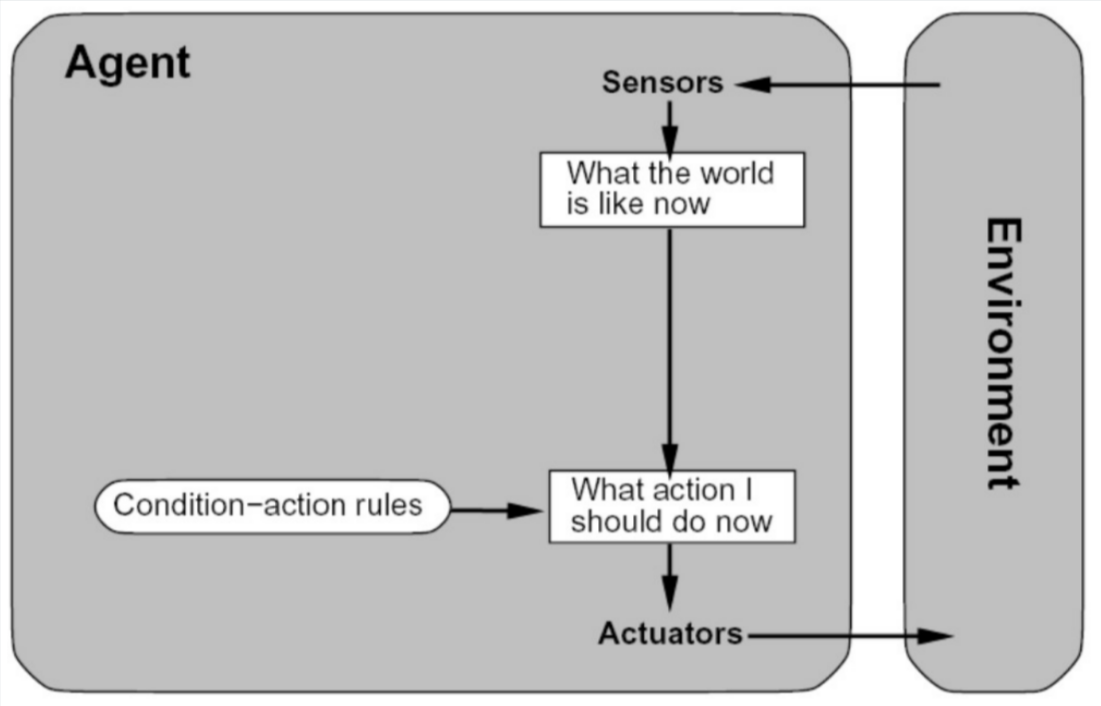
\includegraphics[width=16cm, scale=1]{Images/Imagenes/AgenteReflexoSimple.png}
  \caption{Agente reflexo simple}
\end{figure}

\subsubsection*{Agente reflexo con estado interno}
Tiene un estado interno que le permite
\begin{itemize}
  \item Ver como cambia el ambiente independientemente del agente
  \item Como afectan sus acciones al ambiente (osea tiene memoria)
\end{itemize}

\begin{figure}
  \centering
  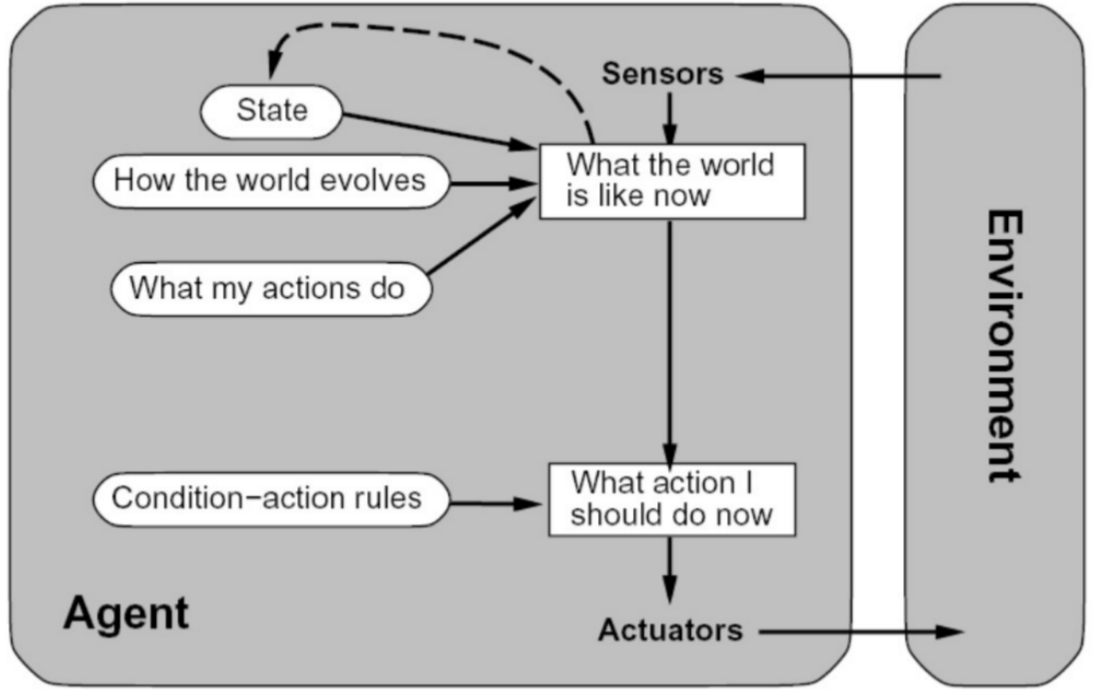
\includegraphics[width=16cm, scale=1]{Images/Imagenes/AgenteReflexoEst.png}
  \caption{Agente reflexo con estado interno}
\end{figure}

\subsubsection*{Agente orientado a metas}
\begin{itemize}
  \item Necesita información de sus metas para escoger que acciones las pueden cumplir
  \item Pueden usarse técnicas de búsqueda y planificación
  \item Esto lo puede hacer mas flexible. Por ejemplo si esta lloviendo ajustar la efectividad de los frenos. Básicamente analiza que es lo que hacen (pero no evalua que tan buenas son) sus posibles acciones para decidir si lo acercan o no a su meta, esto quiere decir que buscan un objetivo sin importarle el como (osea le chupa un huevo la eficiencia solo quiere cumplir su objetivo)
\end{itemize}

\begin{figure}
  \centering
  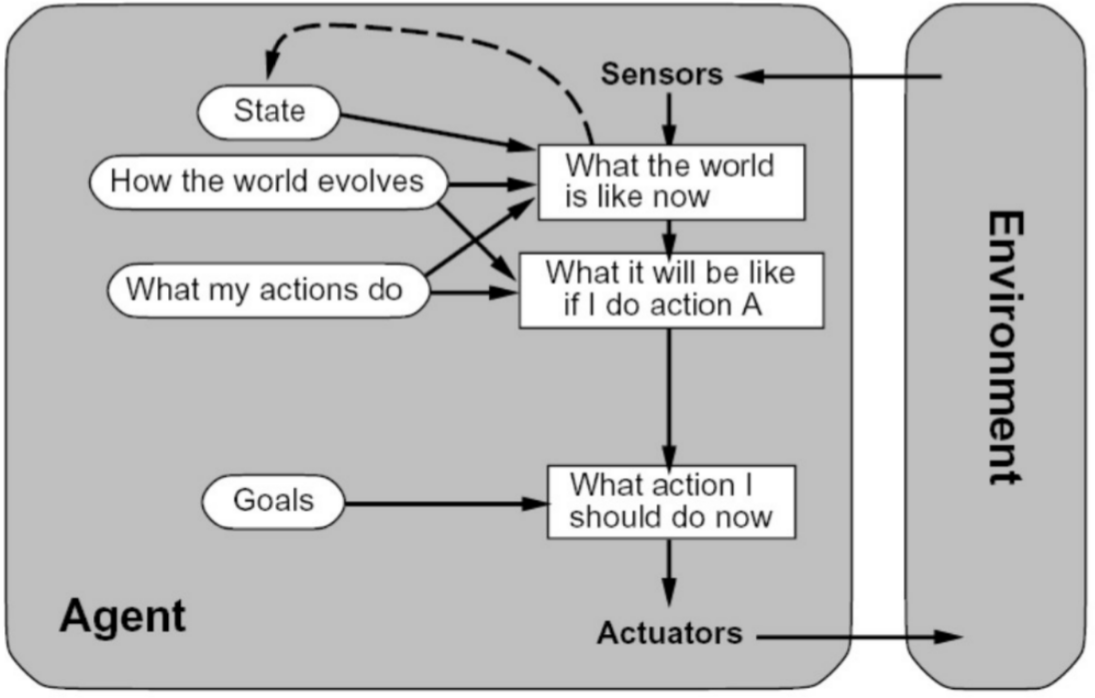
\includegraphics[width=16cm, scale=1]{Images/Imagenes/AgenteOrientadoAMetas.png}
  \caption{Agente orientado a metas}
\end{figure}

\subsubsection*{Agente orientado a la utilidad}
\begin{itemize}
  \item Las metas por si solas no son suficientes para generar un comportamiento de buena calidad (a este no le chupa un huevo la eficiencia :D)
  \item Para esto se necesita una medida de utilidad (función que mapea un estado o secuencia de estados con un numero real).básicamente tiene una función que le tira un numerito que dice que tan buena es la acción para ver si la toma o no.
\end{itemize}

\begin{figure}
  \centering
  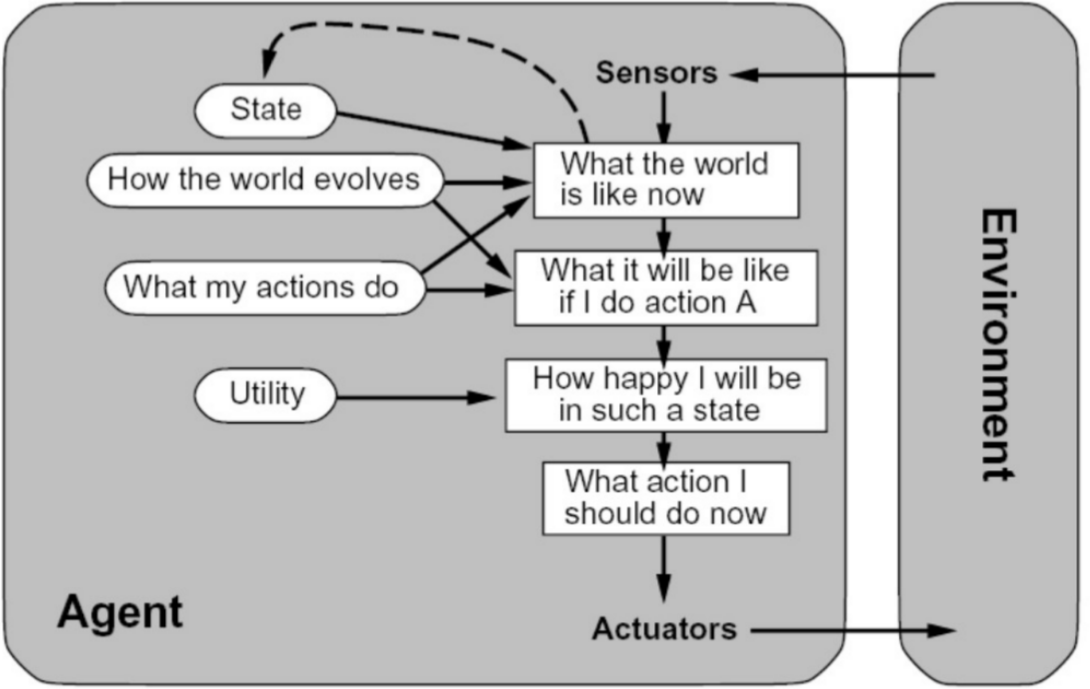
\includegraphics[width=16cm, scale=1]{Images/Imagenes/AgenteOrientadoAutilidad.png}
  \caption{Agente orientado a utilidad}
\end{figure}

\subsubsection*{Agentes que aprenden}
La idea es que las percepciones no se usen solo para actuar, sino también para mejorar su desempeño en el futuro (osea es critico consigo mismo, evalúa constantemente sus acciones y como afectaron al entorno buscando evolucionar y mejorar)

\begin{figure}
  \centering
  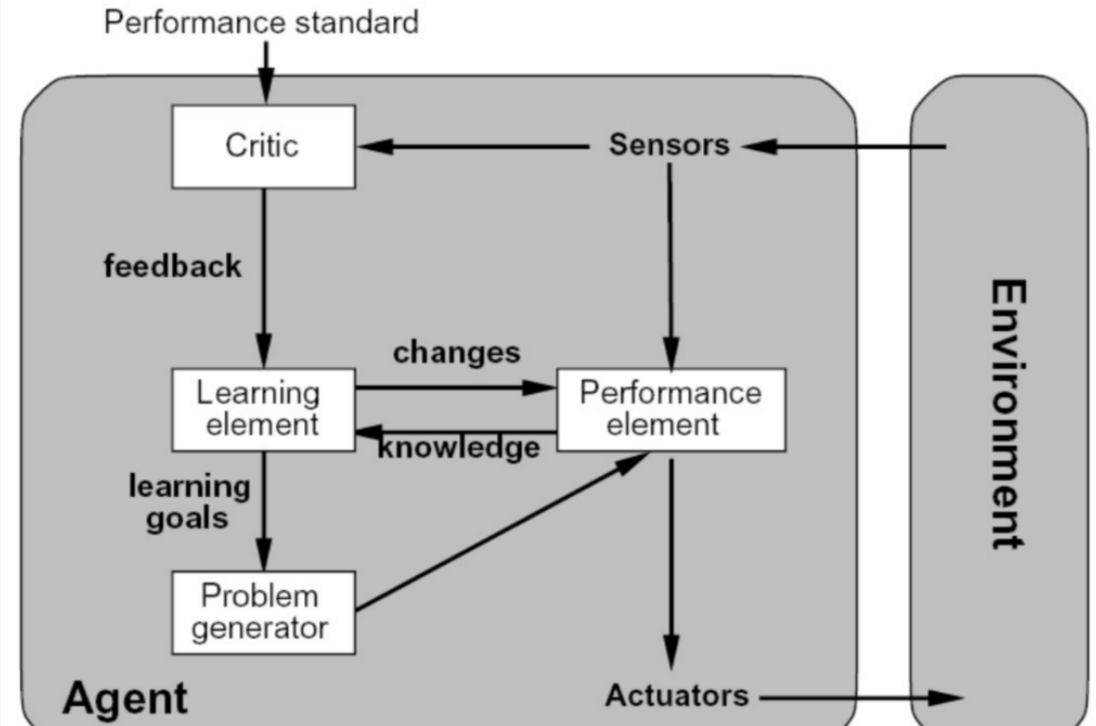
\includegraphics[width=16cm, scale=1]{Images/Imagenes/AgenteQueAprende.png}
  \caption{Agente que aprende}
\end{figure}

\subsubsection*{Inteligencia artificial distribuida-DAI}
\todo[inline]{esto da la sensacion de que no lo preguntan o que ni importa, pero si, con entender que es un sist. multiagente y como interactuan entre si alcanza}
Es el estudio, construcción y aplicación de sistemas multiagente, esto es, sistemas en los cuales varios agentes inteligentes interactúan persiguiendo algún conjunto de objetivos o ejecutando algún conjunto de tareas. Un sistema multiagente es uno que consiste de un numero de agentes, que interactúan entre ellos. En el caso mas general los agentes actúan en favor de sus usuarios con diferentes metas y motivaciones

\textbf{Como interactuan los agentes multiagente}
\begin{itemize}
  \item Coordinación: orientada a la meta o la tarea a realizar ej. cuando dos agentes requieren de un recurso.
  \item Cooperación: varios agentes tratan de combinar sus esfuerzos para lograr un objetivo en grupo. Ningún agente puede en forma solitaria lograr el objetivo, o bien, la cooperación hace obtener mejores resultados ej. obtener resultados en forma mas rápida
  \item Competición: varios agentes tratan de obtener lo que solo algunos de ellos pueden tener
  \item Negociación: varios agentes tratan de obtener su mayor beneficio logrando un acuerdo. Típicamente involucra una oferta contraoferta, con compromisos hechos por los participantes 
\end{itemize}

\subsubsection*{Resumen de que es un agente inteligente}
Son entidades que:
\begin{itemize}
  \item perciben el ambiente
  \item actúan en el
  \item razonan
  \item se comunican con otros agentes
\end{itemize}
Es capaz de acciones autónomas flexibles, es decir:
\begin{itemize}
  \item \textbf{Reactividad: }son capaces de percibir su ambiente y responde a cambios que ocurren
  \item \textbf{Pro-actividad: }son capaces de exhibir funcionamiento orientado a un objetivo, tomando la iniciativa
  \item \textbf{Habilidad social: }son capaces de interactuar con otros agentes (o humanos)
\end{itemize}

\subsection*{Ambientes}
\subsubsection*{Completamente observable vs Parcialmente observable}

Un ambiente es completamente observable si los sensores del agente detectan todos los aspectos relevantes para decidir que acción debe llevarse a cabo. ej Poker seria parcialmente observable y Ajedrez completamente observable

\subsubsection*{Deterministico vs Estocastico}

Si el siguiente estado del ambiente esta completamente determinado por el estado actual y la acción ejecutada por el agente, el ambiente es deterministico. Si otros factores influyen en el proximo estado del ambiente, este es estocástico. ej. jugando al ajedrez el proximo estado del ambiente va a estar determinado por el estado actual y la pieza que se elija mover. Jugando a los dados no esta determinado el proximo estado del ambiente por la acción que realice el agente u el estado actual del ambiente (hay un factor aleatorio que afecta) por lo tanto es estocástico.

\subsubsection*{Agente único vs multiagente}

Un ambiente multiagente es un contexto en el cual multiples agentes interaccionan entre si con su entorno. En un agente único hay un solo agente que toma decisiones y realiza acciones sobre el entorno 

Los ambientes multiagente pueden ser los nombrados mas arriba

\subsubsection*{Episodico vs Secuencial}
En un ambiente episódico, la experiencia del agente esta dividida en episodios atómicos. En cada episodio, el agente percibe y ejecuta una acción simple y el siguiente episodio no depende de las acciones tomadas en episodios anteriores. Ej. Girar una ruleta seria episodico ya que el ambiente no se va a ver afectado por las tiradas anteriores, solo por la accion. Mover una pieza en ajedrez seria secuencial, ya que el nuevo estado depende de las acciones realizadas previamente

\subsubsection*{Discreto vs Continuo}
Esta distinción se aplica al estado del ambiente, al modo en que se maneja el tiempo y a las percepciones y acciones del agente. ej. el tablero de ajedrez es un ambiente discreto. Cada casilla del tablero representa una posición única, y hay un numero finito y discreto de piezas en juego. Cada movimiento del juego es una acción discreta, ya que el agente selecciona una casilla especifica para mover una pieza. Un robot manipulador industrial trabaja en un ambiente continuo, ya que puede mover su brazo y herramienta en una gama infinita de posiciones y orientaciones en el espacio tridimensional. Las acciones para controlar el robot se realizan de manera continua

\subsubsection*{Conocido vs No conocido}
Se refiere mas al estado de conocimiento del agente sobre las leyes o reglas del ambiente. Diferente de parcial-completamente observable. Ej. el solitario es parcialmente observable pero conozco las reglas, por lo tanto es conocido


%Agregar apendice
%\appendix

%Imprimir bibliografia indicada en biblio.bib
\printbibliography

%Mostrar todas las citas sin referenciarlas
%\nocite{*}
\end{document}